
%使用xelatex编译
%版权所有,翻版必究
%本文件由程序自动生成,任何修改将被覆盖
%2019 年 01 月 09 日




\FloatBarrier
\section{
使用C{\sourcefonttwo{}+}{\sourcefonttwo{}+}扩展Qt Quick
}\label{s100710}


读者可能认为使用Qt Quick只需要Qml足以,但不久读者就会失望。
即使退一步,希望Qt Quick可以满足绝大多数需求,这也是难以达成。

Qt Quick不是一种全面代替Qt C{\sourcefonttwo{}+}{\sourcefonttwo{}+}无所不包的解决方案。
Qt Quick只是导出Qt C{\sourcefonttwo{}+}{\sourcefonttwo{}+}的一套接口规范。

当读者面对一个具体的问题,在Qt Quick中无法找到现成的组件或者无法通过
简单修改现有Qt Quick组件达成目的时。使用Qt C{\sourcefonttwo{}+}{\sourcefonttwo{}+}自定义组件就势在必行。

\begin{itemize}

\item 如果所需的组件不需要几何逻辑,
比如实现一个本地文件监视器,那么只继承自QObject即可;

\item 如果所需的组件需要几何逻辑但无需渲染,
比如实现一个鼠标监视器,那么只需要继承自QQuickItem;

\item 如果所需的组件需要渲染,
那么需要继承自QQuickItem,并在构造函数中设置
QQuickItem::ItemHasContents标志位;

\item 如果希望使用QPainter实现渲染,
那么需要继承自QQuickPaintedItem是一个好的选择;

\item 如果仅需要一个简易的OpenGL离屏渲染环境,
那么继承自QQuickFramebufferObject是一个好的选择;

\end{itemize}

如\figurename\ \ref{p000010}
,列出了C{\sourcefonttwo{}+}{\sourcefonttwo{}+}导出Qt Quick基类继承关系图。



%begin图片
\begin{figure}[htb] %浮动体 here and top ...
%there must use marginnote not use marginpar ...
\marginnote{\setlength\fboxsep{2pt}\fbox{\footnotesize{\kaishu\figurename\,}\footnotesize{\ref{p000010}}}}\centering %中心对齐
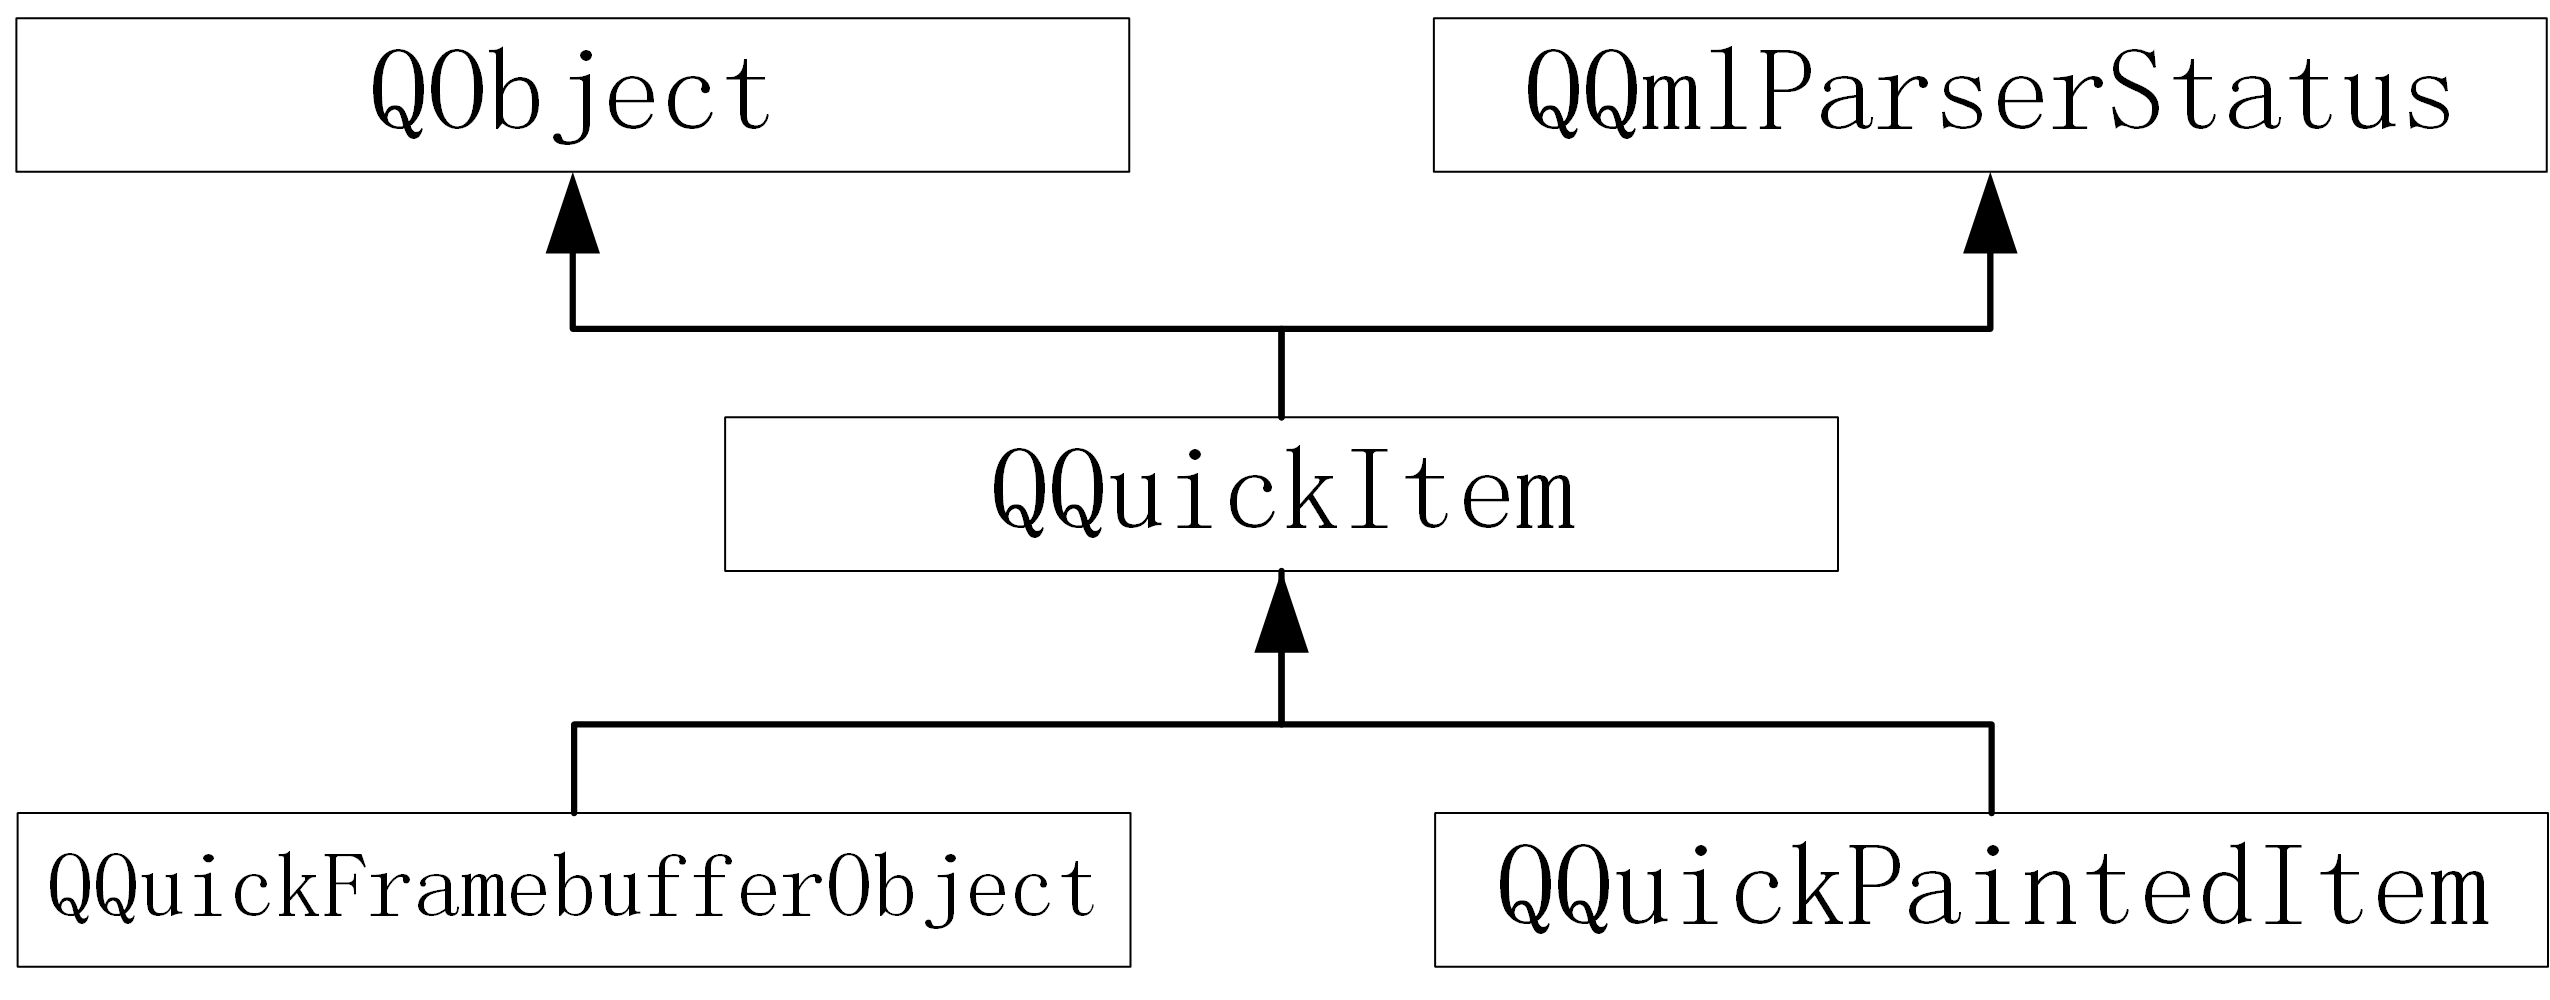
\includegraphics[width=0.95\textwidth]{chapter01/images/qtquick_item.png} %图片路径
\caption{C{\sourcefonttwo{}+}{\sourcefonttwo{}+}导出Qt Quick所需基类} %标题
\label{p000010} %索引
\end{figure}
%end图片







%使用xelatex编译
%版权所有,翻版必究
%本文件由程序自动生成,任何修改将被覆盖
%2019 年 01 月 09 日



